\documentclass{article}
\usepackage[utf8]{inputenc}

\title{Logistic Regression Problems}
\author{Huy Tr.}
\date{October 3rd, 2016}
\usepackage{amsmath}
\usepackage{tikz,pgfplots}
\usepackage{algpseudocode}

\begin{document}

\maketitle

In the previous post, we learned \textbf{Linear Regression} to predict a continuous value by using a linear function as a base line that fit to the data distribution. Now we take another problem: \textbf{classification} and let's see what is the different between this two types.

\section{The Rune Checking Problem}

\begin{flushleft}
So, we have the problem in a DotA 2 match:
\end{flushleft}

\begin{flushleft}
\textit{Sven} joined the battle as an member of the Radiant, who has around 1500 MMR, so he start with a \textit{450} gold boot and took the middle lane, which should belongs to \textit{Pudge}.
\end{flushleft}

\begin{flushleft}
The nightmare didn't stop here, during the match, he left his lane to check for runes in the river every \textit{0.2} minutes!
\end{flushleft}

\begin{flushleft}
Here is the check log that Sven made during his early game:
\end{flushleft}

\begin{table}[h]
\centering
\caption{Sven's Rune Checklog}
\label{rune-check-table}
\begin{tabular}{|l|c|}
\hline
Check Time & Found Rune \\
\hline
1.0        & No         \\
1.2        & No         \\
1.3        & No         \\
1.4        & No         \\
1.6        & No         \\
1.8        & Yes        \\
1.9        & Yes        \\
2.0        & Yes        \\
2.1        & Yes        \\
2.2        & Yes        \\
2.3        & Yes        \\
2.4        & Yes        \\
\hline
\end{tabular}
\end{table}

\begin{flushleft}
Let's take a look at the plot of this check log:
\end{flushleft}

\begin{center}
\begin{tikzpicture}
\begin{axis}[%
scatter/classes={%
    a={mark=o,draw=black}}]
\addplot[scatter,only marks,%
    scatter src=explicit symbolic]%
table[meta=label] {
x   y label
1.0 0 a
1.2 0 a
1.3 0 a
1.4 0 a
1.6 0 a
1.8 1 a
1.9 1 a
2.0 1 a
2.1 1 a
2.2 1 a
2.3 1 a
2.4 1 a
    };
\end{axis}
\end{tikzpicture}
\end{center}

\begin{flushleft}
In order to keep the match from being ruined by Sven's ignorance, we need to help him figure out when is the best time to check for runes, so he don't waste too much time travelling to the river again.
\end{flushleft}

\begin{flushleft}
The idea is to write a computer program that Sven can use at any time, this program will take the current match time and tell him now is a \textbf{good time} or \textbf{bad time} to go check for the runes.
\end{flushleft}

\section{The Classification}

\begin{flushleft}
The problem as described above should be called \textbf{classification}, since we only have a limit number of answers and the predict function should always return one of the answers.
\end{flushleft}

\begin{flushleft}
For example, with \textbf{binary classification}, the \textit{y} values should only takes 0 (\textbf{negative class}) and 1 (\textbf{positive class}).
\end{flushleft}

\begin{flushleft}
Classification can also be found in \textit{spam detection}, \textit{document classification}, \textit{object recognition}, \textit{etc}...
\end{flushleft}

\section{Logistic Regression}

\begin{flushleft}
Logistic Regression is the approach to solve classification by ignoring the fact that \textit{y} is discrete-valued and use the old good \textbf{linear regression} algorithm to predict \textit{y} by \textit{x}. But we need to change our \textbf{hypothesis function} $h_{\theta}(x)$:
\end{flushleft}

\begin{equation}
    h_{\theta}(x)=g(\theta^{T}x)=\frac{1}{1 + e^{-\theta^{T}x}}
\end{equation}

Which: 

\begin{equation}
    g(z)=\frac{1}{1 + e^{-z}}
\end{equation}

Note that:

\begin{equation}
    z = \theta_{0} + \theta_{1}x
\end{equation}

\begin{flushleft}
This called \textbf{logistic function} or \textbf{sigmoid function}
\end{flushleft}

\begin{center}
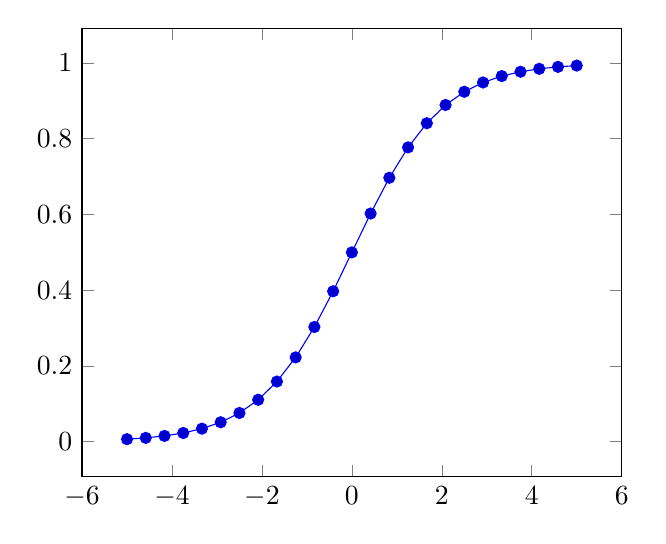
\begin{tikzpicture}
\begin{axis}
\addplot {1/(1 + exp(-x))};
\end{axis}
\end{tikzpicture}
\end{center}

\begin{flushleft}
Notice that $g(z)$ tends towards 1 as $z\rightarrow\infty$ and towards 0 as $z\rightarrow-\infty$, and $g(z)$ (or $h(x)$ as well) is always bounded between 0 and 1.
\end{flushleft}

\begin{flushleft}
We also have the \textbf{derivative of the sigmoid function} as follow:
\end{flushleft}

\begin{equation}
    g'(z)=\frac{d}{dz}\frac{1}{1 + e^{-z}}=g(z)(1 - g(z))
\end{equation}

\section{Optimizing with Gradient Descent}

\begin{flushleft}
We can use the same \textbf{Gradient Descent Algorithm} as we used in \textbf{Linear Regression} to solve \textbf{Logistic Regression} problem.
\end{flushleft}

\begin{flushleft}
For example, this is the \textbf{Stochastic Gradient Descent} algorithm:
\end{flushleft}

\begin{algorithmic}
\Loop
    \For{i $\rightarrow$ m}
        \For{every j}
            $\theta_{j} = \theta_{j} + \alpha(h_{\theta}(x^{(i)}) - y^{(i)})x_{j}$
        \EndFor
    \EndFor
\EndLoop
\end{algorithmic}

\section{Solving Rune Checking Problem with Logistic Regression}

\begin{flushleft}
Now, let's get back to our \textbf{Rune Checking} problem and see how can we use \textbf{Logistic Regression} to solve it.
\end{flushleft}

\begin{flushleft}
Starting with our data, we define a \textbf{hypothesis function} as a \textbf{sigmoid function}
\end{flushleft}

\begin{equation}
    h(x) = \frac{1}{1 + e^{-(\theta_{0} + \theta_{1}x)}}
\end{equation}

\begin{center}
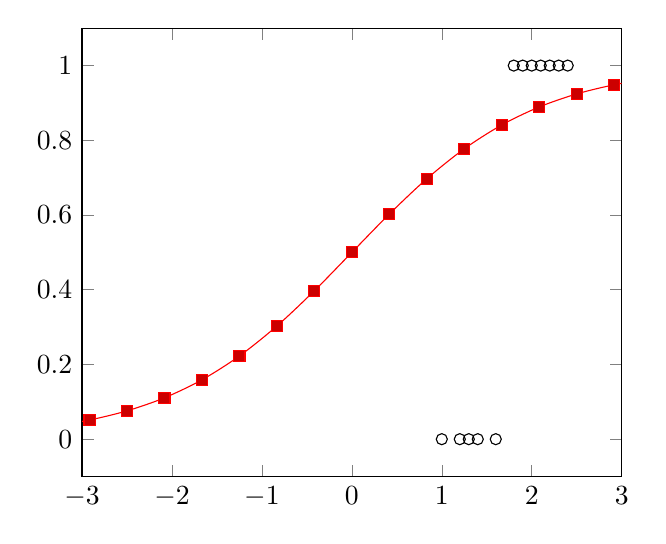
\begin{tikzpicture}
\begin{axis}[%
    xmin=-3, xmax=3,
    scatter/classes={%
        a={mark=o,draw=black}
    },
    ]
\addplot[scatter,only marks,%
    scatter src=explicit symbolic]%
table[meta=label] {
x   y label
1.0 0 a
1.2 0 a
1.3 0 a
1.4 0 a
1.6 0 a
1.8 1 a
1.9 1 a
2.0 1 a
2.1 1 a
2.2 1 a
2.3 1 a
2.4 1 a
};
\addplot+[smooth] {1/(1 + exp(-x))};
\end{axis}
\end{tikzpicture}
\end{center}

\begin{flushleft}
What we need to do is fitting this function to our data, in the other words, we optimizing $\theta_{0}$ and $\theta_{1}$ to make the function become like the following plot:
\end{flushleft}

\begin{center}
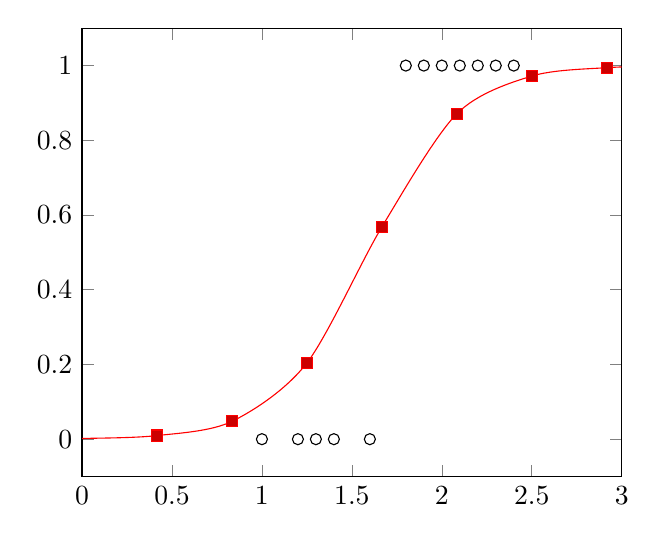
\begin{tikzpicture}
\begin{axis}[%
    xmin=0, xmax=3,
    scatter/classes={%
        a={mark=o,draw=black}
    },
    ]
\addplot[scatter,only marks,%
    scatter src=explicit symbolic]%
table[meta=label] {
x   y label
1.0 0 a
1.2 0 a
1.3 0 a
1.4 0 a
1.6 0 a
1.8 1 a
1.9 1 a
2.0 1 a
2.1 1 a
2.2 1 a
2.3 1 a
2.4 1 a
};
\addplot+[smooth] {1/(1 + exp(-(-6.266031 + 3.923966 * x)))};
\end{axis}
\end{tikzpicture}
\end{center}

\begin{flushleft}
By running \textbf{Gradient Descent}, we found that $\theta_{0}=-6.266031$ and $\theta_{1}=3.923966$. This mean our \textbf{hypothesis function} now become:
\end{flushleft}

\begin{equation}
    h(x) = \frac{1}{1 + e^{-(-6.266031 + 3.923966x)}}    
\end{equation}

\begin{flushleft}
Later on, if you feed some $x$ value to this function, you will get the result as number between $0 \rightarrow 1$.
\end{flushleft}
\begin{flushleft}
At the point this number reached $0.5$, it called \textbf{decision boundary}, everything on the left of the \textbf{decision boundary} will be the \textbf{negative class} and on the right will be the \textbf{possitive class}
\end{flushleft}

\begin{center}
\pgfplotsset{
	legend style={anchor=north west},
	area style
}
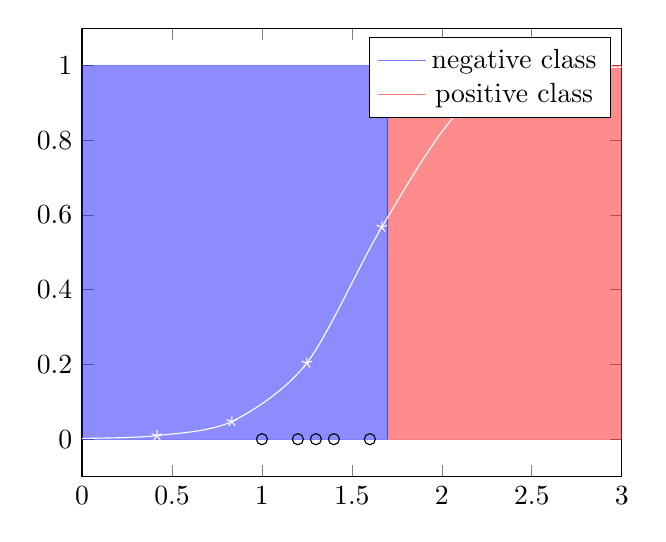
\begin{tikzpicture}
\begin{axis}[%
    xmin=0, xmax=3,
    scatter/classes={%
        a={mark=o,draw=black}
    },
    ]

\addplot[blue,fill=blue!90,opacity=0.5] coordinates {
    (0, 0)
    (1.7, 0)
    (1.7, 1)
    (0, 1)
};
\addlegendentry{negative class}

\addplot[red,fill=red!90,opacity=0.5] coordinates {
    (1.7, 0)
    (3, 0)
    (3, 1)
    (1.7, 1)
};
\addlegendentry{positive class}
    
\addplot[scatter,only marks,%
    scatter src=explicit symbolic]%
table[meta=label] {
x   y label
1.0 0 a
1.2 0 a
1.3 0 a
1.4 0 a
1.6 0 a
1.8 1 a
1.9 1 a
2.0 1 a
2.1 1 a
2.2 1 a
2.3 1 a
2.4 1 a
};
\addplot+[white,smooth,fill=none] {1/(1 + exp(-(-6.266031 + 3.923966 * x)))};
\end{axis}
\end{tikzpicture}
\end{center}

\begin{flushleft}
In the \textbf{Rune Checking} problem, if the given time is in the \textbf{positive} zone, so it's a \textbf{good time} to go for rune, otherwise, it's a \textbf{bad time}, don't go anywhere.
\end{flushleft}

\end{document}
